En esta práctica trabajaremos con árboles parcialmente ordenados (APOs o montículos), con árboles B y con otros árboles vistos en prácticas anteriores.

Para poder realizar esta práctica vamos a poner como ficheros de cabeceras:
\begin{minted}[breaklines]{C++}
  #include <iostream>
  #include "abin.h"
  #include "agen.h"
  #include <vector> //para algunos ejercicios
  #include <string.h> //para algunso ejercicios
\end{minted}

\textbf{\large\underbar{Ejercicio 1:}}\textit{ Dado un árbol binario de enteros donde el valor de cada nodo es menor que el de sus hijos, implementa un subprograma para eliminar un valor del mismo preservando la propiedad de orden establecida. Explica razonadamente la elección de la estructura de datos.}

\underbar{Nota:} Se supone que en el árbol no hay elementos repetidos, y que el número de nodos del mismo no está acotado.

Según el enunciado tenemos un Abin que se comporta como un ABB debido a que el valor de los nodos que son descendientes son mayores que el del padre.
Además si queremos que al eliminar cualquier nodo el árbol siga cumpliendo la propiedad de orden y sabiendo que no podemos eliminar un nodo que no sea hoja, tendremos que intercambiarlo por el nodo cuyo valor sea el menor de los dos hasta que el nodo a eliminar sea una hoja.

Por tanto, nuestra función tendrá como parámetros de entrada el elemento del nodo (para poder buscarlo), el nodo (para poder trabajar con él) y el árbol.
\begin{minted}[breaklines]{C++}
//Métodos auxiliares
template <typename T> bool dosHijos(typename Abin<T>::nodo n, Abin<T> &A){
  return (A.hijoIzqdo(n)!=Abin<T>::NODO_NULO && A.hijoDrcho(n)!=Abin<T>::NODO_NULO);
}

template <typename T> bool esHoja (typename Abin<T>::nodo n, const Abin<T> &A){
  return (A.hijoIzqdo(n) == Abin<T>::NODO_NULO && A.hijoDrcho(n) == Abin<T>::NODO_NULO);
}

template <typename T> Abin<T>::nodo minimo (typename Abin<T>::nodo a,typename Abin<T>::nodo a const Abin<T> &A){
  if(a == Abin<T>::NODO_NULO) return b;
  if(b == Abin<T>::NODO_NULO) return a;
  else return (A.elemento(a) < A.elemento(b)) ? a : b;
}

template <typename T> void eliminar (const T& e, const Abin<T> &A){
  eliminar_rec(e, A.raiz(), A);
}
template <typename T> void eliminar_rec(const T& e, typename Abin<T>::nodo n, Abin<T> &A){
  if(n != Abin<T>::NODO_NULO){
    //Buscamos el nodo que tenga ese elemento
    if(A.elemento(n) == e){
      if(!esHoja(n,A)){
        //Si no es una hoja puede tener 1 ó 2 hijos
        if(dosHijos(n,A)){
          //Si tiene ambos hijos, intercambiamos con el menor de los 2 y el otro pasa a ser hijo
          typename Abin<T>::nodo hijo = minimo(A.hijoIzqdo(n),A.hijoDrcho(n),A);
          A.elemento(n) = A.elemento(hijo);
          eliminar_rec(A.elemento(hijo),hijo,A); //seguimos bajando
        }
        else{ //tiene 1 (puede ser el izquierdo o derecho)
          typename Abin<T>::nodo hijo = (A.hijoIzqdo(n) != Abin<T>::NODO_NULO) ? A.hijoIzqdo(n) : A.hijoDrcho(n);
          A.elemento(n) = A.elemento(hijo);
          eliminar_rec(A.elemento(hijo),hijo,A); //seguimos bajando
        }
      }
      else{
        //es hoja, eliminamos el Nodo
        typename Abin<T>::nodo padre = A.padre(n);
        if (A.hijoIzqdo(padre) == n) {
            A.eliminarHijoIzqdo(padre);
        } else {
            A.eliminarHijoDrcho(padre);
        }
      }
      }else {
        // Seguir buscando en los hijos
        eliminar_rec(e, A.hijoIzqdo(n), A);
        eliminar_rec(e, A.hijoDrcho(n), A);
      }
    //Si es nulo, no hace nada
  }
}

\end{minted}

\textbf{\large\underbar{Ejercicio 2:}}\textit{ Un montículo min-max tiene una estructura similar a la de un montículo ordinario (árbol parcialmente ordenado), pero la ordenación parcial consiste en que los elementos que se encuentran en un nivel par (0, 2, 4,..) son menores o iguales que sus elementos descendientes, mientras que los elementos que se encuentran en un nivel impar (1, 3, 5,..) son mayores o iguales que sus descendientes. Esto quiere decir que para cualquier elemento e de un nivel par se cumple abuelo \(\leq\) e \(\leq\) padre y para cualquier elemento e de un nivel impar padre \(\leq\) e \(\leq\) abuelo.\\
Implementa una operación de orden logarítmico para añadir un elemento a un montículo min-max almacenado en un vector de posiciones relativas.}

Vamos a insertar ese elemento al final del APO, y lo iremos flotando hasta que se quede en la posición correta, por tanto tendremos que realizar una modificación en la función \texttt{flotar()}, ya que como hemos dicho antes, insertarémos por el final del APO.

\begin{minted}[breaklines]{C++}
template <typename T> void APOmM<T>::insertar(const T& e){
  assert(ultimo < maxNodos-1); //APOMinMax no lleno
  nodos[++ultimo] = e; //insertarmos al final e incrementamos el númoero de elementos.
  if(ultimo > 0)
    flotar(ultimo); //reordenamos el APO.
}

template <typename T> void APOmM<T>::flotar(nodo i){
  size_t profundidad = log2(i+1);
  T e = nodos[i];
  T aux;
  nodo abuelo;
  //como i no es raiz, tiene padre
  if(profundidad % 2 == 0){//nivel par
    if(nodos[padre(i)] < nodos[i]){ //Tenemos que reordenar respecto a los niveles impares
      Intercambio(nodos[i],nodos[padre(i)]);
      i = padre(i);
      profundidad--;
      abuelo = padre(padre(i));
      while(abuelo >= 0 && nodos[abuelo] < nodos[i]){
        Intercambio(nodos[i],nodos[abuelo]);
        i = abuelo;
        abuelo = padre(padre(i));
        profundidad-=2;
      }
    }
    else{ //Comprobamos si tenemos que reordenar respecto a los niveles pares del APO.
      abuelo = padre(padre(i));
      while(abuelo >= 0 && nodos[abuelo] > nodos[i]){
        Intercambio(nodos[abuelo],nodos[i]);
        i = abuelo;
        abuelo = padre(padre(i));
        profundidad-=2;
      }
    }
  }else{//nivel impar
    if(padre(i) >= 0 && nodos[padre(i)] > nodos[i]){//Tenemos que reordenar respecto a los niveles pares
      Intercambio(nodos[i],nodos[padre(i)]);
        i = padre(i);
        profundidad--;
        abuelo = padre(padre(i));
        while(abuelo >= 0 && nodos[abuelo] > nodos[i]){
          Intercambio(nodos[i],nodos[abuelo]);
          i = abuelo;
          abuelo = padre(padre(i));
          profundidad-=2;
        }
    }
    else{//Comprobamos si tenemos que reordenar respecto a los niveles pares del APO.
      abuelo = padre(padre(i));
      while(abuelo >= 0 && nodos[abuelo] < nodos[i]){//Reordenamos respecto niveles pares
        Intercambio(nodos[abuelo], nodos[i]);
        i = abuelo;
        abuelo = padre(padre(i));
        profundidad-=2;
      }
    }
  }
}
\end{minted}

\textbf{\large\underbar{Ejercicio 3:}}\textit{ Implementa una operación de orden logarítmico para eliminar el elemento máximo de un montículo min-max definido como en el problema anterior.}

\begin{minted}[breaklines]{C++}
template <typename T> void APOmM::suprimirMax(){
  assert(ultimo > -1);
  if(--ultimo > -1){//APO no queda vacío
    if(ultimo >= 2){//Tiene dos hijos y al menos 1 nieto, el máximo está en uno de los 2 hijos.
      if(nodos[1] > nodos[2]){
        nodos[1] = nodos[ultimo+1];
        hundir(1);
      }else{
        nodos[2] = nodo[ultimo+1];
        hundir(2);
      }
    }else if(ultimo == 1){
      nodos[1] == std::min(nodos[1],nodos[2])M
    }
  }
}
\end{minted}

\textbf{\large\underbar{Ejercicio 4:}}\textit{ Un árbol es estrictamente ternario si todos sus nodos son hojas o tienen tres hijos. Escribe una función que, dado un árbol de grado arbitrario, nos indique si es o no estrictamente ternario.}

Vamos a partir de un Agen, ya que son los únicos que pueden tener más de dos hijos (un hijo izquierdo y los hermanos de este).

\begin{minted}[breaklines]{C++}
template <typename T> bool esTernario(const Agen<T> &A){
  return esTernario_rec(A.raiz(), A);
}

template <typename T> bool esTernario_rec(typename Agen<T>::nodo n, const Agen<T> &A){
  //n es un nodo nulo
  if(n == Agen<T>::NODO_NULO)
    return true;
  //n no tiene hijos.
  else if(A.hijoIzqdo(n) == Agen<T>::NODO_NULO && A.hermDrcho(n)== Agen<T>::NODO_NULO)
    return true;
  //n tiene hijos
  else if(A.hijoIzqdo(n) != Agen<T>::NODO_NULO && A.hermDrcho(n)!= Agen<T>::NODO_NULO){
    //llamamos a la función para sus hijos
    esTernario_rec(A.hijoIzqdo(n),A) && esTernario_rec(A.hermDrcho(n),A);
  }
  else //Tiene 1 hijo.
    return false;
}
\end{minted}

\textbf{\large\underbar{Ejercicio 5:}}\textit{ Una forma de representar una figura plana en blanco y negro consiste en utilizar un árbol cuaternario en el que cada nodo o tiene exactamente cuatro hijos, o bien es una hoja. Un nodo hoja puede ser blanco o negro y un nodo interno no tiene color.}

Una figura dibujada dentro de un cuadrado de lado 2k se representa de la forma siguiente: Se divide el cuadrado en cuatro cuadrantes y cada uno se representa como un hijo del nodo raíz. Si un cuadrante está completamente negro corresponde a una hoja negra; si, por el contrario, el cuadrante está completamente blanco, éste corresponde a una hoja blanca; y si un cuadrante está parcialmente ocupado por negro y blanco, entonces corresponde a un nodo interno del árbol y este cuadrante se representa siguiendo el mismo método subdividiéndolo en otros cuatro cuadrantes. Como ejemplo se muestra una figura en blanco y negro y su árbol asociado, tomando los cuadrantes en el sentido de las agujas del reloj a partir del cuadrante superior izquierdo.
\begin{figure}[h]
  \begin{center}
    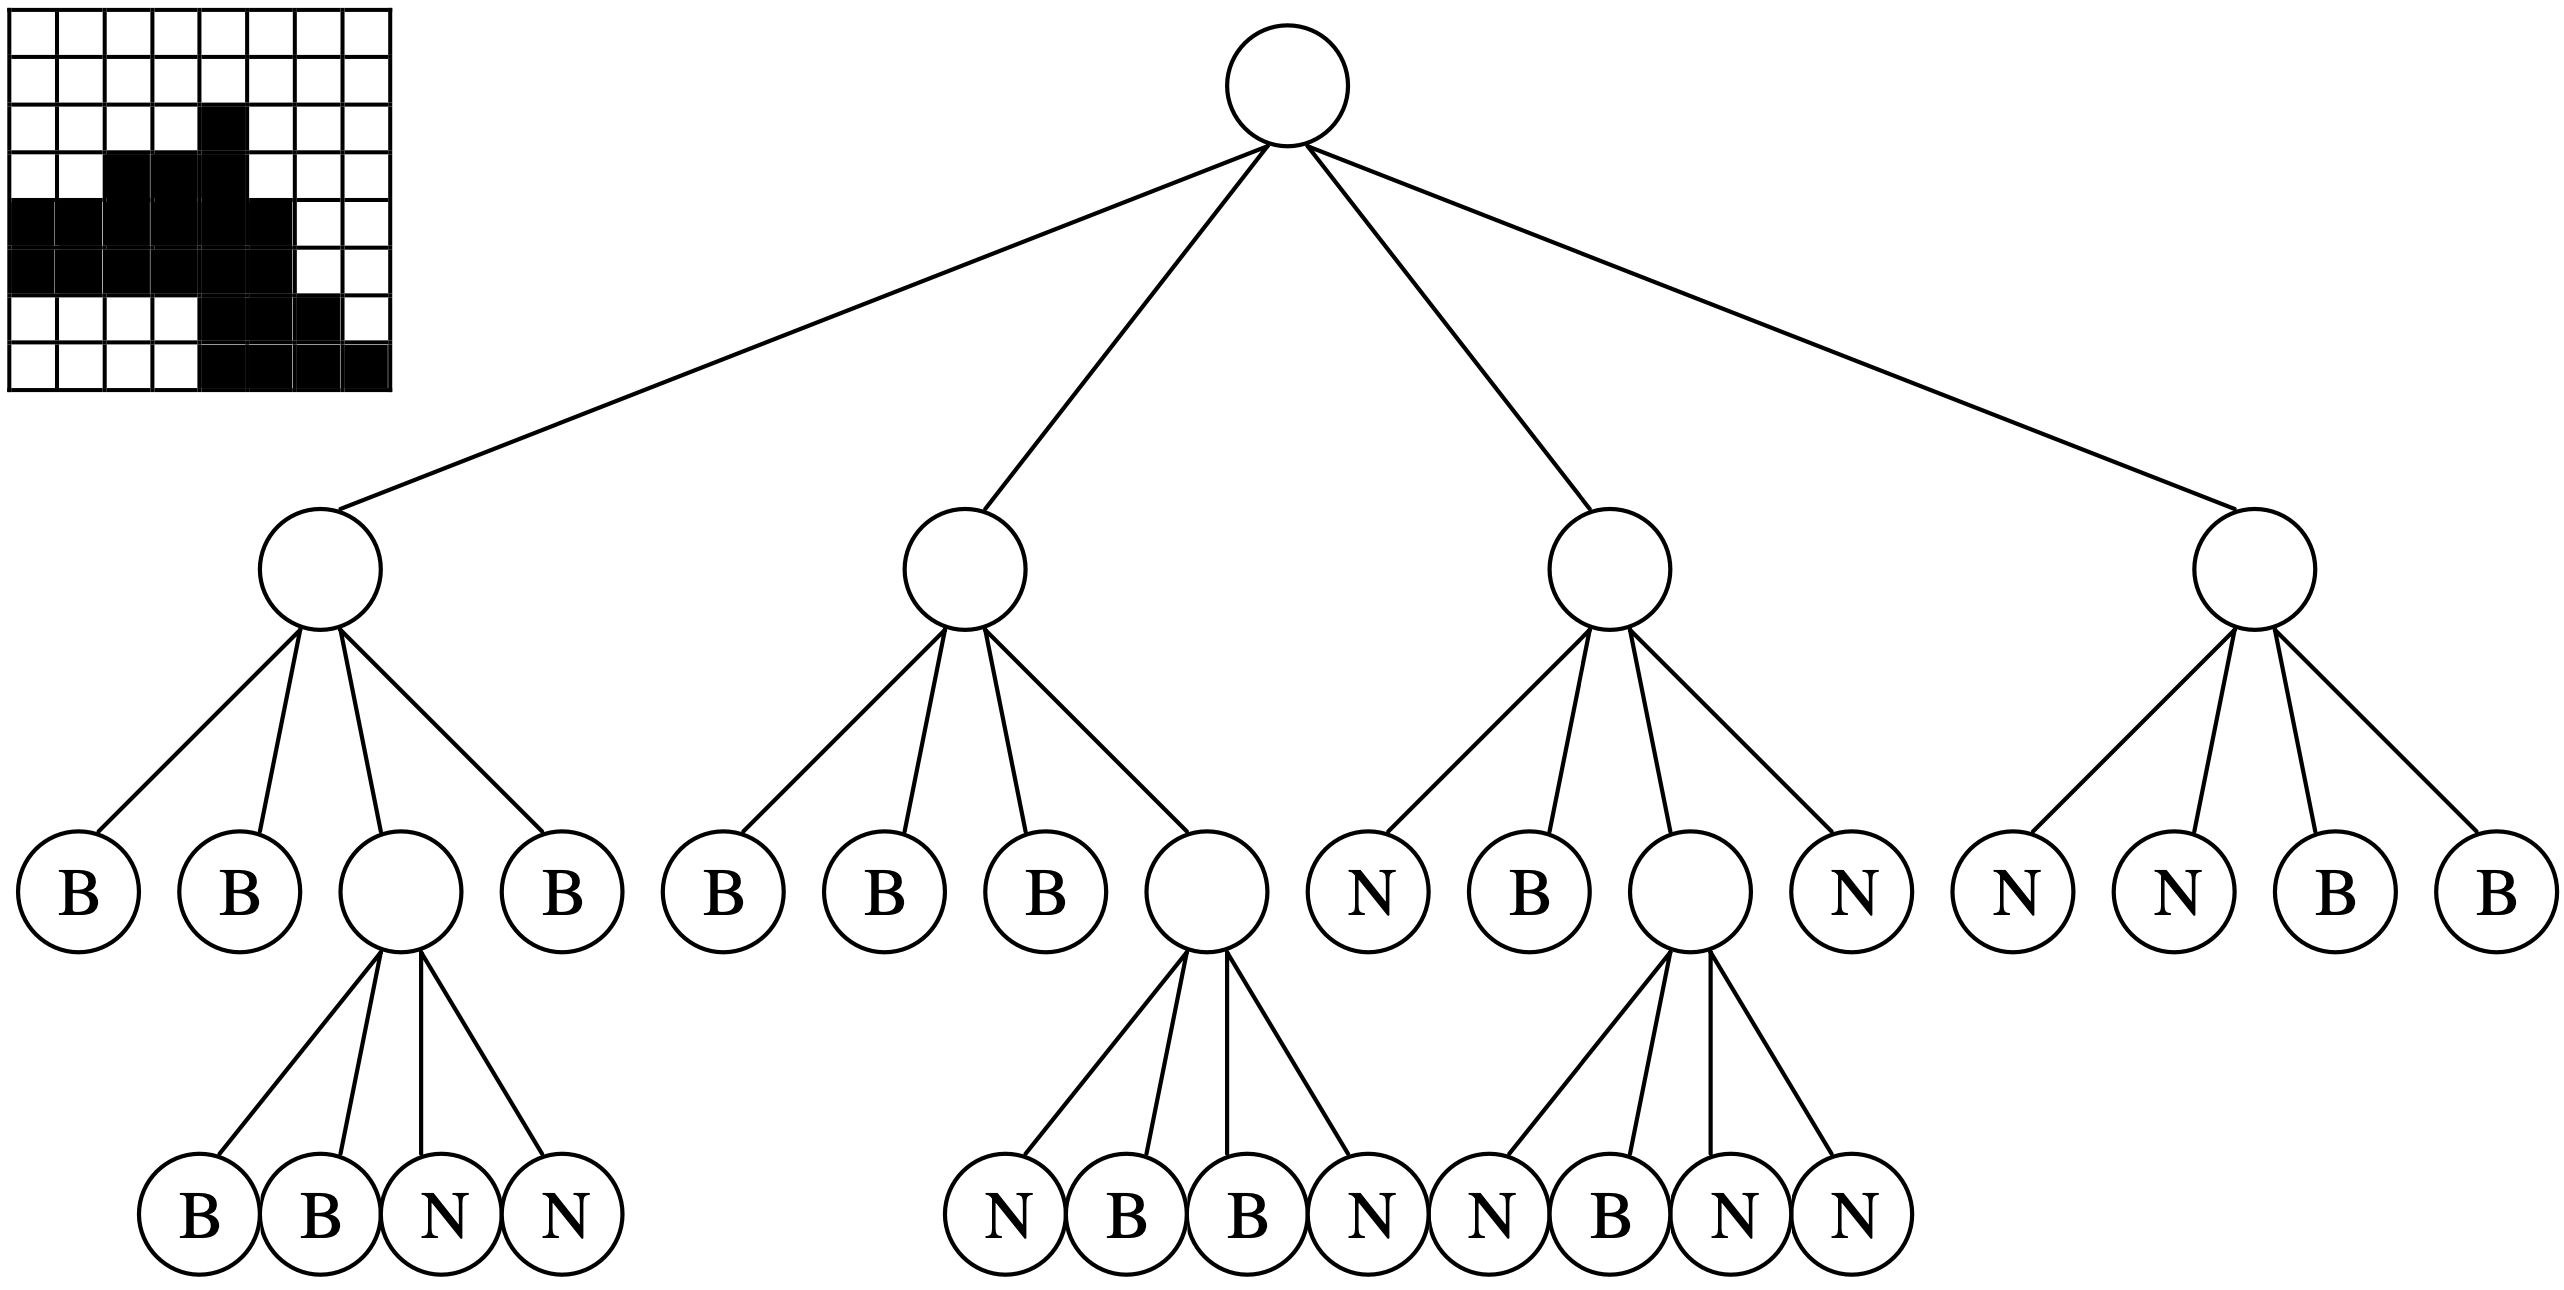
\includegraphics[width=.7\textwidth]{assets/p5.png}
  \end{center}
\end{figure}

Implementa una función que dado un árbol de esta clase, con k+1 niveles, devuelva la figura asociada, representada como una matriz cuadrada de tamaño 2k en la que cada celda representa un punto blanco o negro.

\underbar{Nota:} Por simplificar el problema, se asume que en cada nodo del árbol se incluyen las coordenadas de la esquina superior izquierda y de la esquina inferior derecha del cuadrante que representa.

Partimos de la base que tenemos un árbol cuaternario (4 hijos por cada nodo) y sabemos que los nodos intermedios están vacios (no tienen un color asociado).
El primer hijo del árbol, es decir, el hijo izquierdo del nodo raíz contempla los primeros cuatro cuadrados de la matriz (arriba a la izquierda), siendo estos todos "blancos" porque no tienen un color asociado.

Sabemos la dimensiones de la matriz que sería \(2k\), es decir \(2*(NumNodos-1)\), en este caso, como tenemos 33 nodos en el árbol, tenemos \(2*(33-1) = 64\) casillas, es decir una matriz de tamaño 8x8 = 64.

Como cada casilla tiene un color asociado o no, podemos creanos una estructura llamada "pixel" la cual contendrá la información de cada casilla junto con su "coordenada".
\begin{minted}[breaklines]{C++}
typedef struct Pixel{
  std::string color; //typedef enum {B,N,V}color;
  int filaS[2]; //fila
  int filaI[2]; //columa
};

//devolvemos la matriz por referencia 
template <typename Pixel> void figura (typename Agen<Pixel>::nodo n, const Agen<Pixel> &A, std::vector<std::vector<Pixel>> &M){
  if(n!= Agen<Pixel>::NODO_NULO){
    if(A.elemento(n).color == " "){ //Nodo intermedio del árbol
      typename Agen<Pixel>::nodo aux = A.hijoIzqdo(n);
      while(aux != Agen<Pixel>::NODO_NULO){
        figura(aux,A,M);
        aux = A.hermDrcho(aux);
      }
    }
    else{ //Tiene color asociado
      if(A.elemento(n).color == "B" || A.elemento(n).color == "N"){
        //Vamos acceder a la posición de la matriz en sentido horario:
        for(auto i = A.elemento(n).filaS[0]; i<= A.elemento(n).filaS[1]; i++)
          for(auto j = A.elemento(n).filaI[1]; j<= A.elemento(n).filaI[0]; j--){
            M[i][j] = A.elemento(n).color;
          }
      }
    }
  }
}
\end{minted}